\documentclass[a4paper,12pt]{article}
\usepackage[utf8]{inputenc}
\usepackage{amsmath}
\usepackage{hyperref}
\usepackage{graphicx}
\usepackage{geometry}
\usepackage{amsfonts}
\usepackage{ulem}
\usepackage{listings}
\usepackage{float}
\lstset{basicstyle=\ttfamily, breaklines=true} % automatische Zeilenumbrüche

\geometry{a4paper, margin=1.3in}

\title{Abgabe 1 für Computergestützte Methoden}
\author{Gruppe 91, Rohan Rasho, Alpay Akcay, Kim Levin Schröder}
\date{\today}

\begin{document}

\newpage
% Titelseite
\maketitle

% Inhaltsverzeichnis
\renewcommand{\contentsname}{Inhaltsangabe}
\tableofcontents
\newpage

% Kapitel 1 - Der zentrale Grenzwertsatz
\section{Der zentrale Grenzwertsatz}
Der zentrale Grenzwertsatz (ZGS) ist ein fundamentales Resultat der Wahrscheinlichkeitstheorie, das die Verteilung von Summen unabhängiger, identisch verteilter (i.i.d.) Zufallsvariablen (ZV) beschreibt. Er besagt, dass unter bestimmten Voraussetzungen die Summe einer großen Anzahl solcher ZV annähernd normalverteilt ist, unabhängig von der Verteilung der einzelnen ZV. Dies ist besonders nützlich, da die Normalverteilung gut untersucht und mathematisch handhabbar ist.

\subsection{Aussage}
Sei $X_1, X_2, \dots, X_n$ eine Folge von i.i.d. ZV mit dem Erwartungswert $\mu = E(X_i)$ und der Varianz $\sigma^2 = \text{Var}(X_i)$, wobei $0 < \sigma^2 < \infty$ gelte. Dann konvergiert die standardisierte Summe $Z_n$ dieser ZV für $n \to \infty$ in Verteilung gegen eine Standardnormalverteilung:\footnote{Der zentrale Grenzwertsatz hat verschiedene Verallgemeinerungen. Eine davon ist der \textbf{Lindeberg-Feller-Zentrale-Grenzwertsatz} [\hyperlink{source1}{1}, Seite 328], der schwächere Bedingungen an die Unabhängigkeit und die identische Verteilung der ZV stellt.}

\begin{equation}
Z_n = \frac{\sum_{i=1}^n X_i - n\mu}{\sigma \sqrt{n}} \xrightarrow{d} N(0, 1).
\end{equation}

\noindent Das bedeutet, dass für große $n$ die Summe der ZV näherungsweise normalverteilt ist mit Erwartungswert $n\mu$ und Varianz $n\sigma^2$:

\begin{equation}
\sum_{i=1}^n X_i \sim N(n\mu, n\sigma^2).
\end{equation}

\subsection{Erklärung der Standardisierung}
Um die Summe der ZV in eine Standardnormalverteilung zu transformieren, subtrahiert man den Erwartungswert $n\mu$ und teilt durch die Standardabweichung $\sigma \sqrt{n}$. Dies führt zu der obigen Formel (1). Die Darstellung (2) ist für $n \to \infty$ nicht wohldefiniert.

\subsection{Anwendungen}
Der ZGS wird in vielen Bereichen der Statistik und der Wahrscheinlichkeitstheorie angewendet. Typische Beispiele sind:

\begin{itemize}
    \item \textbf{Schätzen von Mittelwerten bei Stichproben}: Der zentrale Grenzwertsatz hilft dabei zu verstehen, warum der Durchschnitt von Stichproben einer Normalverteilung folgt, selbst wenn die Grundgesamtheit nicht normalverteilt ist.
    \item \textbf{Analyse großer Datensätze in der Wirtschaft und Naturwissenschaft}: Der zentrale Grenzwertsatz ermöglicht die Anwendung der Normalverteilung auf die Summe vieler kleiner Einflüsse, was in vielen Bereichen der Forschung nützlich ist.
\end{itemize}

% Kapitel 2 - Bearbeitung zur Aufgabe 1
\newpage
\section{Bearbeitung zur Aufgabe 1}
\subsection{Thema Datenverarbeitung} 
\subsubsection {Teilaufgabe 1}: \\ Die uns zugeteilten Daten beinhalten Daten, die im Zusammenhang mit einem Fahrradverleih stehen. Sie umfassen Wetterdaten und Verleihzahlen, aber auch die Station und das Datum für jeden Tag des Jahres 2023. Die Zeilen geben den Datensatz für jeden Jahrestag des Jahres 2023 und für jede Station in Reihenfolge an. Und die Spalten A bis L geben die Attribute in dieser Reihenfolge an "group", "station", "date", "day of year", "day of week", "month of year", "precipitation", "windspeed", "min temperature", "average temperature", "max temperature", "count". Unserer Gruppe 91 wurde die Station "W 56 St & 10 Ave" zugeordnet, für welche wir keinen besonderen Zusammenhang zwischen den Wetterdaten und den Verleihzahlen beobachten können. Jedoch fällt uns auf, dass wir quasi genau die gleichen Wetterdaten und Datumsangaben, wie die anderen Gruppen haben, wobei der einzige Unterschied zwischen den Gruppen ist, dass verschiedene Werte zwischen den Gruppen, in den Spalten, nicht verfügbar "NA" sind, die meisten Werte aber übereinstimmen. Der "Count"  ist stations- bzw. gruppenbedingt unterschiedlich. 
\\
\subsubsection{Teilaufgabe 2}: \\
Um die Daten in Excel zu laden, und mit ihnen arbeiten zu können, haben wir die CSV-Datei in Excel geladen, in dem wir die Daten nach Kommas getrennt haben (Daten $ \rightarrow $ Daten abrufen $ \rightarrow $ Aus Datei $ \rightarrow $ Aus Text/CSV $ \rightarrow $ Trennzeichen=Komma und Datentyperkennung=Basierend auf dem gesamten Dataset $ \rightarrow $Laden). Dies hat die Daten richtig auf die Spalten aufgeteilt. 
\\
\subsubsection{TEilaufgabe 3}: \\Danach haben wir „group“ angeklickt und nur Gruppe 91 ausgewählt. Damit Excel die Zahlen als numerische Werte behandelt und uns keine 0 als Lösung liefert, haben wir die Zelle J angeklickt, da hier die Durchschnittstemperatur „average temperature“ enthalten ist und haben dann den Textkonvertierungsassistenten genutzt (Daten $ \rightarrow $ Text in Spalten $ \rightarrow $ Fertig stellen).  Nun geben wir in einer freien Zelle den Befehl "=MAX(J:J)" ein, welcher uns das Ergebnis 83 geliefert hat. Vermutlich ist dieser Wert in Grad Fahrenheit angegeben, da dies amerikanische Wetterdaten, vermutlich aus New York, sind. Um dies in Grad Celsius umzurechnen, haben wir in eine freie Zelle den Befehl "=(N32805-32)* 5/9" angegeben, welcher uns den Wert 28,3 °C liefert. 
\begin{figure}[H]
    \centering
    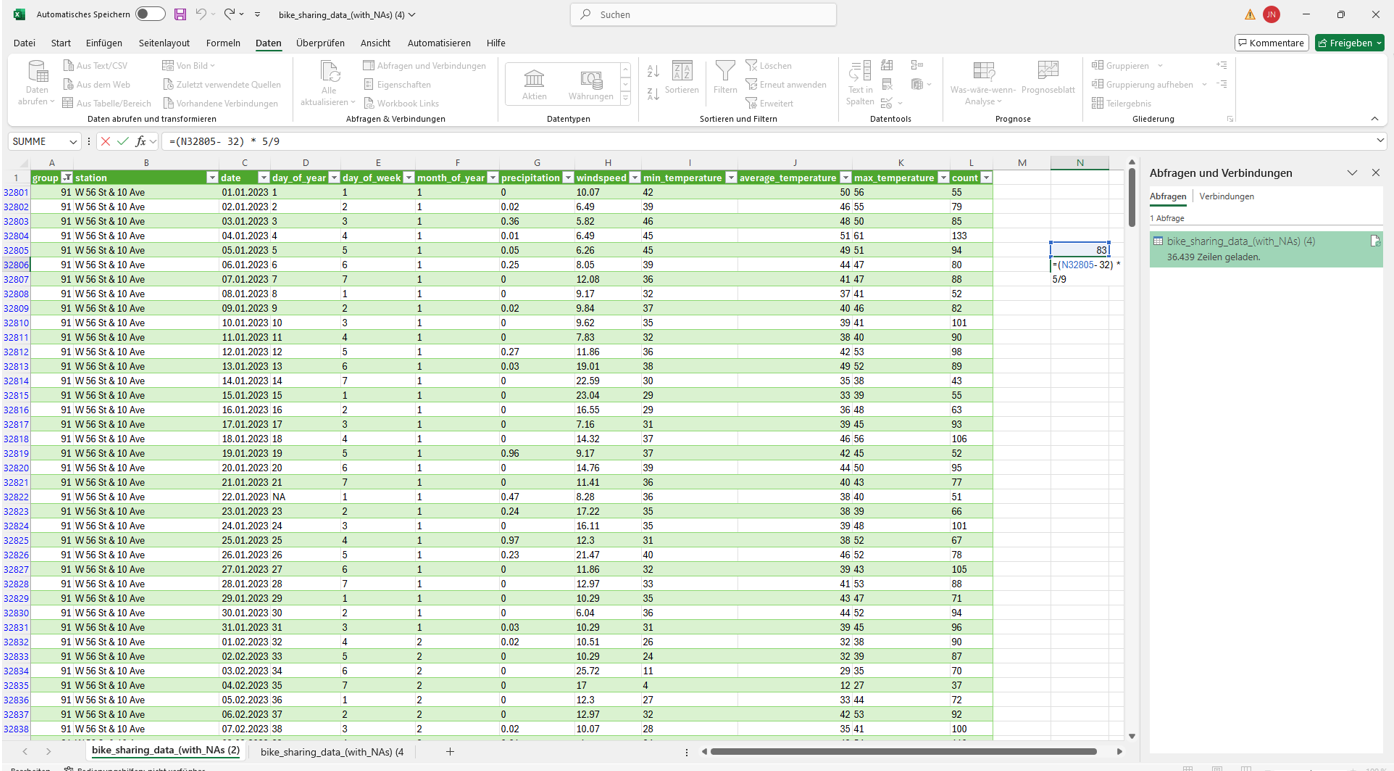
\includegraphics[width=\textwidth]{image2.png}
    \caption{Enter Caption}
    \label{fig:enter-label}
\end{figure}
\subsection{Thema Datenhaltung} 
\subsubsection{Teilaufgabe 2}:\\ In unserer Datenbank sind, bis auf die zusammengesetzte Adresse "station", nur atomare Werte verwendet worden. Die Stationsadresse betrachten wir dennoch als atomaren Wert und trennen nicht nach Straßen bzw.  Hausnummern, da Adressen in New York meist nach Kreuzungen angegeben werden und uns dies keine weitere Hilfe bezüglich der Bearbeitung liefert. Außerdem wäre es auch schwer eine einheitliche Trennung zu finden, da hier nicht immer "\&" als Trennzeichen der Kreuzungsstraßen verwendet wird, sondern manchmal auch \\"-" oder auch Adressen wie "Washington Square E" gegeben sind, was sich nicht trennen lässt. Somit ist die erste Normalform quasi gegeben. \\ \\
Datenbank-Schema:\\
Verleih(\uline{ID\#}, Jahrestag\#, StationID\#, WetterdatenID\#, Count)\\ \\
Wetterdaten(\uline{WetterdatenID\#}, Niederschlag, Windgeschwindigkeit, Tiefsttemperatur, Durchschnittstemperatur, Höchsttemperatur)\\ \\
Stationen(\uline{StationID\#}, Adresse)\\ \\
Kalenderdatum(\uline{Jahrestag\#}, Datum, Wochentag, Monatstag)\\ \\
"\_": Primärschlüssel\\
"\#“: Schlüsselattribute (auch Fremdschlüssel)\\ \\
Diese Datenbank befindet sich in zweiten Normalform, da zusätzlich zur ersten Normalform gegeben ist, dass alle Nichtschlüssel-Attribute nur vom Primärschlüssel abhängig sind, nicht aber von einer Teilmenge desselben. 
\\

\subsubsection{Teilaufgabe 3}:\\
Sql-Eingaben: 
\begin{lstlisting}
.open Fahrradverleih.db
PRAGMA foreign_keys = ON;
CREATE TABLE Wetterdaten (WetterdatenID int primary key, Niederschlag real, Windgeschwindigkeit real, Tiefsttemperatur int, Durchschnittstemperatur int, Hoechsttemperatur int);
CREATE TABLE Stationen (StationID int primary key, Adresse text);
CREATE TABLE Kalenderdatum (Jahrestag int primary key, Datum Text, Wochentag int, Monatstag int);
CREATE TABLE Verleih (ID int primary key, Jahrestag int, StationID int, WetterdatenID int, count int, 
FOREIGN KEY(Jahrestag) REFERENCES Kalenderdatum(Jahrestag), 
FOREIGN KEY(StationID) REFERENCES Stationen(StationID), 
FOREIGN KEY(WetterdatenID) REFERENCES Wetterdaten(WetterdatenID));
\end{lstlisting}
\\ \subsubsection{Teilaufgabe 4}: \\
Das Vorbereiten der Datensätze haben wir in Excel durchgeführt, in dem wir den gegebenen Datensatz verändert haben. Hierbei haben wir für die Tabelle "Stationen", die "group"-Spalte und die "station"-Spalte ausgewählt und die restlichen gelöscht. Dann haben wir die Dublikate mit dem dafür zuständigen Excelbefehl entfernt, woraufhin wir "group" zu "StationenID" umbenannt haben. \\ \\
Im nächsten Schritt haben wir für die Tabelle Kalenderdatum alle nicht Datumsabhängigen Spalten gelöscht, die restlichen sortiert, und alle redundanten Zeilen gelöscht, sodass nur noch 365 übriggeblieben sind. In den Spalten suchten wir nach "NA" und haben diese Werte durch die richtigen ersetzt.\\ \\
Als Nächstes haben wir die Wetterdaten Tabelle erstellt, in dem wir für jede Zelle eine WetterdatenID nach Nummerierung erstellt haben (in erster Zeile 1 und in zweiter Zeile 2 eingeben, markieren und auf weitere Zeilen erweitern). Wir haben hier nicht auf 365 Werte reduziert aufgrund der verschiedenen "NA"s, die wir nicht wie beim Datum ausgelöscht haben und da es für unsere spätere Bearbeitung nicht bedeutsam ist. Wir haben wieder alle nicht relevanten Spalten gelöscht und die restlichen in Schema-Reihenfolge gebracht.\\ \\
Zum Schluss haben wir die Tabelle Verleih erstellt, in dem wir eine ID-Spalte wie bei der WetterdatenID eingefügt haben, die Schlüssel der anderen Tabellen eingefügt haben und tabellenspezifisch die gleichen Schritte wie oben durchgeführt haben. Um die "NA"s in der Jahrestag-Spalte zu entfernen, haben wir den Befehl "=WENN(D2="NA";D1\+1;D2)" genutzt, die Spaltenwerte fixiert und die Ursprungsspalte "day of year", auf die die Funktion verweist, gelöscht.\\ \\
Zuletzt haben wir die Tabellen jeweils in eigenen CSV-Dateien mit Semikolon als Trennzeichen in Excel gespeichert, weswegen wir in SQL den Separator anpassen.\\ \\

\noindent Der SQL-Code zur Datenimportierung lautet wie folgt: \\ 

\noindent .separator ; \\ \\
.import Stationen.csv Stationen\\ \\
.import Wetterdaten1.csv Wetterdaten \\ \\
.import Kalenderdatum.csv Kalenderdatum \\ \\
.import Verleih.csv Verleih \\ 

\subsubsection{Teilaufgabe 5}: \\ Der SQL-Code zur Abfrage der gruppenspezifischen höchsten Durchschnittstemperatur lautet wie folgt:\\ \\
\begin{lstlisting}
SELECT MAX((Wetterdaten.Durchschnittstemperatur - 32) * 5 / 9) AS  HoechsteDurchschnittstemperatur_Celsius
FROM Verleih 
INNER JOIN Wetterdaten ON Verleih.WetterdatenID = Wetterdaten.WetterdatenID
 AND  Wetterdaten.Durchschnittstemperatur != 'NA'; 
 \end{lstlisting}
\\ \\
\noindent Beweis der Funktionstüchtigkeit des Codes: 
\begin{figure}[H]
    \centering
    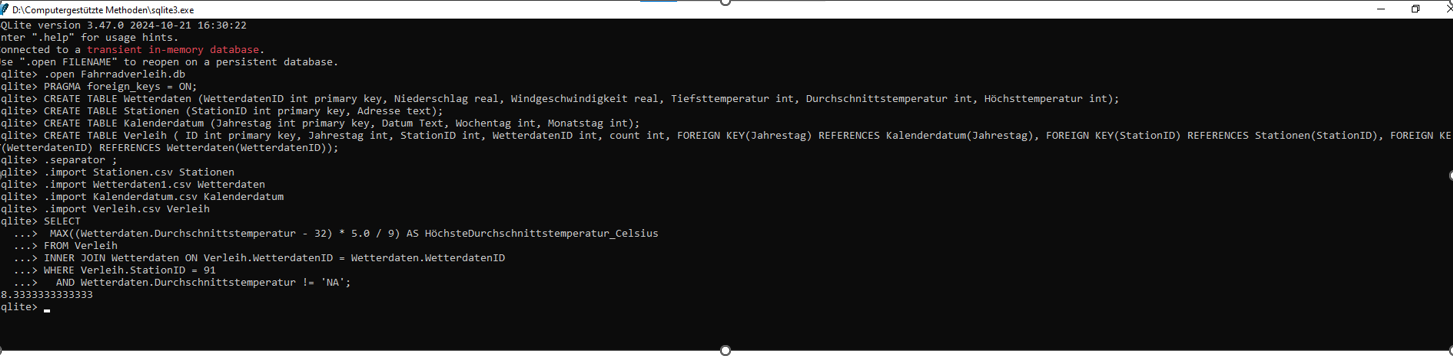
\includegraphics[width=\textwidth]{image.png}

    \label{fig:enter-label}
\end{figure}
\noindent Hier kann man auch erkennen, dass uns Sqlite für unsere Gruppe die höchste Durchschnittstemperatur von 28.3 °C liefert.








% Literaturverzeichnis
\newpage
\renewcommand{\refname}{Literatur}
\begin{thebibliography}{9}
    \bibitem{source1} \hypertarget{source1}{} Achim Klenke. \textit{Wahrscheinlichkeitstheorie}. Springer, 3. Auflage, 2013.
   
\end{thebibliography}

\end{document}
